\documentclass[11pt,a4paper]{article}

% --- Core Packages ---
\usepackage[utf8]{inputenc}
\usepackage[T1]{fontenc}
\usepackage{amsmath, amssymb, amsfonts, amsthm}
\usepackage{geometry}
\usepackage{xcolor}
\usepackage{graphicx}
\usepackage{booktabs}
\usepackage{array}
\usepackage{enumitem}
\usepackage{fancyhdr}
\usepackage{sectsty}
\usepackage[colorlinks=true, linkcolor=RoyalBlue, citecolor=RoyalBlue, urlcolor=RoyalBlue]{hyperref}

% --- TikZ Setup for Diagrams ---
\usepackage{tikz}
\usetikzlibrary{arrows.meta, positioning, calc}

% --- Elegant Styling & Boxes ---
\usepackage[most]{tcolorbox}

% Define Theme Colors
\definecolor{RoyalBlue}{rgb}{0.08, 0.35, 0.65}
\definecolor{DarkSlate}{rgb}{0.15, 0.20, 0.25}
\definecolor{CrimsonRed}{rgb}{0.75, 0.10, 0.15}
\definecolor{ForestGreen}{rgb}{0.10, 0.55, 0.20}
\definecolor{Eggplant}{rgb}{0.38, 0.12, 0.38}
\definecolor{SoftGray}{rgb}{0.96, 0.97, 0.98}
\definecolor{dimgray}{rgb}{0.41, 0.41, 0.41}

% Apply Margins
\geometry{
    top=1.0in,
    bottom=1.0in,
    left=0.85in,
    right=0.85in,
    headheight=14pt
}

% Section and Subsection Fonts
\sectionfont{\color{RoyalBlue}\sectionrule{0pt}{0pt}{-5pt}{1pt}}
\subsectionfont{\color{Eggplant}}
\subsubsectionfont{\color{DarkSlate}}

% Headers and Footers
\pagestyle{fancy}
\fancyhf{}
\fancyhead[L]{\color{gray}\itshape Electricity \& Magnetism --- One-Shot Revision Notes}
\fancyhead[R]{\color{gray}\itshape Revision Guide}
\fancyfoot[C]{\thepage}
\renewcommand{\headrulewidth}{0.4pt}

% --- Styled Custom TColorBoxes ---
\newtcolorbox{formulabox}[1][]{
    enhanced,
    colback=SoftGray,
    colframe=RoyalBlue,
    width=\textwidth,
    arc=4mm,
    boxrule=1.5pt,
    title=\textbf{#1},
    coltitle=white,
    colbacktitle=RoyalBlue,
    attach boxed title to top left={yshift=-2mm, xshift=5mm},
    boxed title style={arc=1.5mm},
    fonttitle=\sffamily\bfseries,
    drop shadow={RoyalBlue!20!white}
}

\newtcolorbox{pyqbox}[1][]{
    enhanced,
    colback=white,
    colframe=CrimsonRed,
    width=\textwidth,
    arc=2mm,
    boxrule=1.2pt,
    title=\textbf{#1},
    coltitle=white,
    colbacktitle=CrimsonRed,
    attach boxed title to top left={yshift=-2mm, xshift=5mm},
    boxed title style={arc=1mm},
    fonttitle=\sffamily\bfseries\small,
    drop shadow={CrimsonRed!15!white}
}

\newtcolorbox{prioritybox}[1][]{
    enhanced,
    colback=RoyalBlue!5!white,
    colframe=RoyalBlue!80!black,
    width=\textwidth,
    arc=3mm,
    boxrule=1.5pt,
    title=\textbf{#1},
    coltitle=white,
    colbacktitle=RoyalBlue!80!black,
    attach boxed title to top left={yshift=-2.5mm, xshift=5mm},
    boxed title style={arc=1.5mm},
    fonttitle=\sffamily\bfseries,
    drop shadow={RoyalBlue!15!white}
}

\newtcolorbox{successbox}[1][]{
    enhanced,
    colback=ForestGreen!5!white,
    colframe=ForestGreen,
    width=\textwidth,
    arc=2mm,
    boxrule=1pt,
    fontupper=\sffamily\bfseries\color{ForestGreen},
    halign=center
}

\begin{document}

% --- Elegant Cover / Title Page ---
\begin{titlepage}
    \centering
    \vspace*{2cm}
    {\Huge\bfseries\color{RoyalBlue} Electricity \& Magnetism}\\[0.6cm]
    {\Large\bfseries\color{Eggplant} One-Shot Revision Notes (Serial Wise)}\\[1.5cm]
    \rule{\linewidth}{1.5pt}\\[1.5cm]
    
    \begin{tcolorbox}[colback=RoyalBlue!5!white, colframe=RoyalBlue, arc=4mm, boxrule=1pt, halign=center, width=0.85\linewidth]
        \large\sffamily\color{DarkSlate}
        \textbf{Exam Revision Version --- High Yield Notes} \\[0.3cm]
        Contains formulas, definitions, crucial derivations, TikZ diagrams, and high-weightage topics curated directly from PYQs.
    \end{tcolorbox}
    
    \vfill
    {\large \textbf{Designed for Quick Revision \& Exam Readiness}}\\[0.2cm]
    {\large \today}
    \vspace*{1cm}
\end{titlepage}

\tableofcontents
\newpage

% =========================================================================
% PART 1: ELECTROSTATICS
% =========================================================================
\section{Part 1: Electrostatics}

\begin{tcolorbox}[colback=yellow!10!white, colframe=orange, arc=2mm, boxrule=1pt]
    \sffamily\small\textbf{Important Note:} This is the condensed exam-oriented revision version. Focus heavily on memorizing the boxed formulas, definitions, and high-weightage derivations listed under the PYQ sections.
\end{tcolorbox}

\subsection{Electric Charge}
Electric charge is the fundamental intrinsic property of matter that gives rise to electric forces.

\subsubsection{Key Properties}
\begin{enumerate}
    \item \textbf{Quantization of Charge:} Charge exists only in discrete integral multiples of the elementary charge $e$.
    \begin{formulabox}[Quantization of Charge]
        \[ q = ne \]
        Where $e = 1.6 \times 10^{-19}\text{ C}$ is the charge of a proton/electron, and $n \in \mathbb{Z}$.
    \end{formulabox}
    \item \textbf{Conservation of Charge:} The total net electric charge of an isolated system remains constant over time.
    \item \textbf{Additivity of Charge:} Total charge of a system is the algebraic sum of all individual charges: $q_{\text{total}} = q_1 + q_2 + q_3 + \dots$
\end{enumerate}

\subsection{Coulomb's Law}
Provides the electrostatic force of attraction or repulsion between two stationary point charges.

\begin{center}
    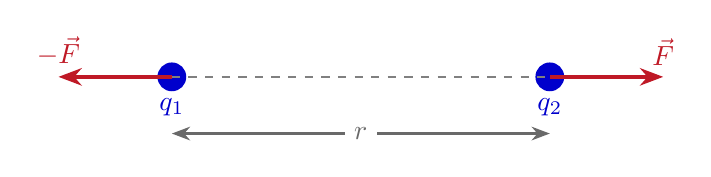
\begin{tikzpicture}[>=Stealth, thick, scale=1.2]
        % Charges
        \filldraw [blue!80!black] (0,0) circle (4pt) node[below=4pt] {$q_1$};
        \filldraw [blue!80!black] (4,0) circle (4pt) node[below=4pt] {$q_2$};
        % Line connecting them
        \draw [dashed, gray] (0,0) -- (4,0);
        % Dimension line
        \draw [<->, dimgray] (0,-0.6) -- (4,-0.6) node[midway, fill=white] {$r$};
        % Force arrow (repulsive example)
        \draw [->, CrimsonRed, very thick] (4,0) -- (5.2,0) node[above] {$\vec{F}$};
        \draw [->, CrimsonRed, very thick] (0,0) -- (-1.2,0) node[above] {$-\vec{F}$};
    \end{tikzpicture}
\end{center}

\begin{formulabox}[Coulomb's Law Formula]
    \[ F = \frac{1}{4\pi\epsilon_0} \frac{q_1 q_2}{r^2} \]
    Where $\epsilon_0$ is the permittivity of free space ($\epsilon_0 = 8.854 \times 10^{-12}\text{ C}^2/\text{N}\cdot\text{m}^2$).
\end{formulabox}

\begin{formulabox}[Electrostatic Constant]
    \[ \frac{1}{4\pi\epsilon_0} = 9 \times 10^9 \text{ N}\cdot\text{m}^2/\text{C}^2 \]
\end{formulabox}

\subsection{Electric Field Intensity}
The electric field intensity $\vec{E}$ at any point is defined as the electrostatic force experienced per unit positive test charge placed at that point.

\begin{formulabox}[Electric Field Strength]
    \[ E = \frac{F}{q} \quad \implies \quad \vec{E} = \frac{\vec{F}}{q} \]
    \textbf{Unit:} $\text{N/C}$ (or $\text{V/m}$)
\end{formulabox}

\subsection{Electric Field Due to a Point Charge}
Determines the electric field produced by a single source charge $+Q$ at a distance $r$.

\begin{center}
    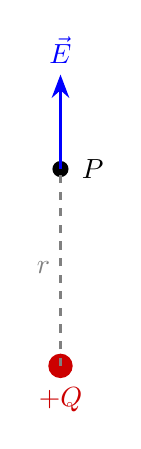
\begin{tikzpicture}[>=Stealth, thick]
        % Charge
        \filldraw [red!80!black] (0,0) circle (4pt) node[below=4pt] {$+Q$};
        % Point P
        \filldraw [black] (0,2.5) circle (2.5pt) node[right=4pt] {$P$};
        % Distance line
        \draw [dashed, gray] (0,0) -- (0,2.5) node[midway, left] {$r$};
        % Field arrow at P
        \draw [->, blue, very thick] (0,2.5) -- (0,3.7) node[above] {$\vec{E}$};
    \end{tikzpicture}
\end{center}

\begin{formulabox}[Electric Field (Point Charge)]
    \[ E = \frac{1}{4\pi\epsilon_0} \frac{Q}{r^2} \]
\end{formulabox}

\subsection{Superposition Principle}
The net electric field at any point due to a system of multiple stationary charges is the vector sum of the electric fields produced by each individual charge at that point.

\begin{formulabox}[Superposition Principle]
    \[ \vec{E}_{\text{net}} = \vec{E}_1 + \vec{E}_2 + \vec{E}_3 + \dots = \sum_{i=1}^n \vec{E}_i \]
\end{formulabox}

\subsection{Electric Flux}
Electric flux is a measure of the number of electric field lines passing through a given surface area $A$.

\begin{formulabox}[Electric Flux Formula]
    \[ \phi_E = \vec{E} \cdot \vec{A} = EA \cos\theta \]
    Where $\theta$ is the angle between the electric field vector $\vec{E}$ and the normal vector to the surface area $\vec{A}$. \\[0.2cm]
    \textbf{Unit:} $\text{N}\cdot\text{m}^2/\text{C}$
\end{formulabox}

\subsubsection{Special Cases}
\begin{itemize}
    \item \textbf{Maximum Flux ($\theta = 0^\circ$):} The field lines are normal to the surface.
    \[ \phi_E = EA \]
    \item \textbf{Zero Flux ($\theta = 90^\circ$):} The field lines run parallel to the surface.
    \[ \phi_E = 0 \]
\end{itemize}

\subsection{Gauss's Theorem}
\begin{pyqbox}[PYQ Priority: \textasteriskcentered\textasteriskcentered\textasteriskcentered\textasteriskcentered\textasteriskcentered]
    \textbf{Statement:} The net electric flux $\phi_E$ through any closed Gaussian surface is equal to $\frac{1}{\epsilon_0}$ times the net charge enclosed within that surface.
\end{pyqbox}

\begin{formulabox}[Gauss's Law (Integral Form)]
    \[ \oint \vec{E} \cdot d\vec{A} = \frac{Q_{\text{enclosed}}}{\epsilon_0} \]
\end{formulabox}

\begin{formulabox}[Gauss's Law (Differential Form)]
    \[ \nabla \cdot \vec{E} = \frac{\rho}{\epsilon_0} \]
    Where $\rho$ is the volume charge density.
\end{formulabox}

\subsection{Applications of Gauss's Law}

\subsubsection{(A) Infinite Line Charge}
\begin{pyqbox}[PYQ Priority: \textasteriskcentered\textasteriskcentered\textasteriskcentered\textasteriskcentered\textasteriskcentered]
    Calculates the electric field at a perpendicular distance $r$ from an infinitely long wire with uniform linear charge density $\lambda$.
\end{pyqbox}

\begin{center}
    \begin{tikzpicture}[>=Stealth, thick]
        % Infinite Line
        \draw [very thick, dimgray] (0,-2.2) -- (0,2.2) node[above] {$\lambda$};
        \foreach \y in {-1.8, -1.2, -0.6, 0, 0.6, 1.2, 1.8} {
            \node[blue, scale=0.8] at (0.2, \y) {$+$};
        }
        % Point P
        \filldraw [black] (2,0) circle (2.5pt) node[right=4pt] {$P$};
        % Distance
        \draw [dashed, gray] (0,0) -- (2,0) node[midway, above] {$r$};
        % Field vector
        \draw [->, blue, very thick] (2,0) -- (3.3,0) node[right] {$\vec{E}$};
    \end{tikzpicture}
\end{center}

\begin{formulabox}[Electric Field of Infinite Line Charge]
    \[ E = \frac{\lambda}{2\pi\epsilon_0 r} \]
\end{formulabox}

\subsubsection{(B) Infinite Plane Sheet}
\begin{pyqbox}[PYQ Priority: \textasteriskcentered\textasteriskcentered\textasteriskcentered\textasteriskcentered\textasteriskcentered]
    Calculates the electric field produced by an infinite plane sheet of charge with uniform surface charge density $\sigma$.
\end{pyqbox}

\begin{formulabox}[Electric Field of Infinite Plane Sheet]
    \[ E = \frac{\sigma}{2\epsilon_0} \]
    \textbf{Crucial Note:} The electric field is completely \textbf{independent of the distance} $r$ from the sheet.
\end{formulabox}

\subsubsection{(C) Uniformly Charged Sphere}
For a solid insulating sphere of radius $R$ and total uniform charge $Q$:
\begin{itemize}
    \item \textbf{Outside the Sphere ($r \ge R$):}
    \begin{formulabox}[Outside Sphere]
        \[ E = \frac{1}{4\pi\epsilon_0} \frac{Q}{r^2} \]
    \end{formulabox}
    \item \textbf{Inside the Sphere ($r < R$):}
    \begin{formulabox}[Inside Sphere]
        \[ E = \frac{1}{4\pi\epsilon_0} \frac{Qr}{R^3} \]
    \end{formulabox}
\end{itemize}

\subsection{Electric Potential}
The electric potential $V$ at any point in an electric field is the amount of work done per unit positive charge in bringing it from infinity to that point against electrostatic forces.

\begin{formulabox}[Electric Potential Formula]
    \[ V = \frac{W}{q} \]
    \textbf{Unit:} $\text{Volt (V)} = \text{J/C}$
\end{formulabox}

\subsection{Potential Due to a Point Charge}
\begin{formulabox}[Potential (Point Charge)]
    \[ V = \frac{1}{4\pi\epsilon_0} \frac{Q}{r} \]
\end{formulabox}

\subsection{Relation Between Electric Field and Potential}
\begin{pyqbox}[PYQ Priority: \textasteriskcentered\textasteriskcentered\textasteriskcentered\textasteriskcentered\textasteriskcentered]
    Defines the relationship between the electric field intensity and the electric potential gradient.
\end{pyqbox}

\begin{formulabox}[Relation Between E and V]
    \[ E = -\frac{dV}{dr} \]
    \textbf{Vector Form (Gradient):}
    \[ \vec{E} = -\nabla V \]
\end{formulabox}

\subsection{Potential Energy}
The electrostatic potential energy $U$ of a charge $q$ in an electric potential $V$ is:
\begin{formulabox}[Potential Energy (Single Charge)]
    \[ U = qV \]
\end{formulabox}

For a system of two point charges $q_1$ and $q_2$ separated by a distance $r$:
\begin{formulabox}[Potential Energy (Two Charges)]
    \[ U = \frac{1}{4\pi\epsilon_0} \frac{q_1 q_2}{r} \]
\end{formulabox}

\subsection{Electric Dipole}
\begin{pyqbox}[PYQ Priority: \textasteriskcentered\textasteriskcentered\textasteriskcentered\textasteriskcentered\textasteriskcentered\ (Direct 10 Marks Derivation)]
    A pair of equal and opposite point charges $+q$ and $-q$ separated by a very small distance $2a$.
\end{pyqbox}

\begin{center}
    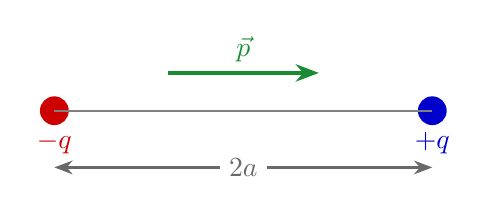
\begin{tikzpicture}[>=Stealth, thick, scale=1.2]
        % Charges
        \filldraw [red!80!black] (-2,0) circle (4pt) node[below=4pt] {$-q$};
        \filldraw [blue!80!black] (2,0) circle (4pt) node[below=4pt] {$+q$};
        % Line
        \draw [thick, gray] (-2,0) -- (2,0);
        % Dimension
        \draw [<->, dimgray] (-2,-0.6) -- (2,-0.6) node[midway, fill=white] {$2a$};
        % Dipole Moment vector (pointing from -q to +q)
        \draw [->, ForestGreen, very thick] (-0.8,0.4) -- (0.8,0.4) node[midway, above] {$\vec{p}$};
    \end{tikzpicture}
\end{center}

\begin{formulabox}[Dipole Moment]
    \[ p = q(2a) \quad \implies \quad \vec{p} = q(2\vec{a}) \]
    The vector direction of $\vec{p}$ is always from the \textbf{negative charge to the positive charge}. \\
    \textbf{Unit:} $\text{C}\cdot\text{m}$
\end{formulabox}

\subsection{Potential Due to an Electric Dipole}
\begin{pyqbox}[PYQ Priority: \textasteriskcentered\textasteriskcentered\textasteriskcentered\textasteriskcentered\textasteriskcentered]
    General formula for the potential $V$ at any position $(r, \theta)$ relative to the dipole center.
\end{pyqbox}

\begin{formulabox}[Potential of a Dipole (General)]
    \[ V = \frac{1}{4\pi\epsilon_0} \frac{p \cos\theta}{r^2} \]
\end{formulabox}

\begin{itemize}
    \item \textbf{Axial Position ($\theta = 0^\circ$):}
    \[ V_{\text{axial}} = \frac{1}{4\pi\epsilon_0} \frac{p}{r^2} \]
    \item \textbf{Equatorial Position ($\theta = 90^\circ$):}
    \[ V_{\text{equatorial}} = 0 \]
\end{itemize}

\subsection{Electric Field Due to a Dipole}

\begin{itemize}
    \item \textbf{Axial Field (End-on Position):}
    \begin{formulabox}[Axial Electric Field]
        \[ E_{\text{axial}} = \frac{1}{4\pi\epsilon_0} \frac{2p}{r^3} \]
    \end{formulabox}
    \item \textbf{Equatorial Field (Broadside-on Position):}
    \begin{formulabox}[Equatorial Electric Field]
        \[ E_{\text{equatorial}} = \frac{1}{4\pi\epsilon_0} \frac{p}{r^3} \]
    \end{formulabox}
    \item \textbf{General Position Field:}
    \begin{formulabox}[General Electric Field]
        \[ E = \frac{1}{4\pi\epsilon_0} \frac{p}{r^3} \sqrt{1 + 3\cos^2\theta} \]
    \end{formulabox}
\end{itemize}

\subsection{Torque on an Electric Dipole}
When placed in a uniform external electric field $\vec{E}$:
\begin{formulabox}[Torque on Dipole]
    \[ \tau = pE \sin\theta \]
    \textbf{Vector Form:}
    \[ \vec{\tau} = \vec{p} \times \vec{E} \]
\end{formulabox}

\subsection{Potential Energy of a Dipole}
The potential energy stored in a dipole placed in a uniform electric field $\vec{E}$:
\begin{formulabox}[Potential Energy of Dipole]
    \[ U = -pE \cos\theta = -\vec{p} \cdot \vec{E} \]
\end{formulabox}

\subsection{Polarization}
The polarization $\vec{P}$ is defined as the induced electric dipole moment per unit volume of a dielectric material.
\begin{formulabox}[Polarization]
    \[ P = \frac{\text{Electric Dipole Moment}}{\text{Volume}} \]
    \textbf{Unit:} $\text{C/m}^2$
\end{formulabox}

\subsection{Relation Between Polarization and Surface Charge Density}
\begin{pyqbox}[PYQ Priority: \textasteriskcentered\textasteriskcentered\textasteriskcentered\textasteriskcentered]
    Relates the polarization vector to the induced surface bound charge density $\sigma_p$.
\end{pyqbox}

\begin{formulabox}[Polarization and Bound Charge]
    \[ \sigma_p = P \]
    \textbf{General Vector Form:}
    \[ \sigma_p = \vec{P} \cdot \hat{n} \]
    Where $\hat{n}$ is the unit normal vector pointing outward from the dielectric surface.
\end{formulabox}

\subsection{Dielectric Constant}
The ratio of permittivity of the medium to the permittivity of free space.
\begin{formulabox}[Dielectric Constant]
    \[ K = \frac{\epsilon}{\epsilon_0} \]
\end{formulabox}

\subsection{Electric Susceptibility}
Measures how easily a dielectric polarizes when subjected to an external electric field.
\begin{formulabox}[Electric Susceptibility]
    \[ \vec{P} = \epsilon_0 \chi_e \vec{E} \]
    Where $\chi_e$ is the dimensionless electric susceptibility.
\end{formulabox}

\subsubsection{Key Relation}
\begin{formulabox}[Relation Between K and Susceptibility]
    \[ K = 1 + \chi_e \]
\end{formulabox}

\subsection{Electric Displacement Vector}
The electric displacement vector $\vec{D}$ accounts for the effects of both free and bound charges in a dielectric material.
\begin{formulabox}[Electric Displacement Vector]
    \[ \vec{D} = \epsilon \vec{E} \]
    \textbf{Alternative Form:}
    \[ \vec{D} = \epsilon_0 \vec{E} + \vec{P} \]
\end{formulabox}

\subsection{Gauss's Law in Dielectrics}
In a dielectric medium, the total flux of the electric displacement vector $\vec{D}$ through any closed surface is equal to the net free charge enclosed within that surface. Bound charges are implicitly accounted for by the polarization term inside $\vec{D}$.
\begin{formulabox}[Gauss's Law in Dielectrics]
    \[ \oint \vec{D} \cdot d\vec{A} = Q_{\text{free}} \]
    \textbf{Differential Form:}
    \[ \nabla \cdot \vec{D} = \rho_{\text{free}} \]
\end{formulabox}

\subsection{Capacitor with Dielectric}
When a dielectric material of dielectric constant $K$ is introduced between the plates of a parallel plate capacitor, its capacitance always increases from $C_0$ to $C = K C_0$. However, other electrical quantities depend on whether the battery remains connected or is isolated.

\begin{enumerate}
    \item \textbf{Case 1: Battery Remains Connected (Voltage Constant)}
    \begin{itemize}
        \item \textbf{Potential Difference:} $V = V_0$ (remains constant).
        \item \textbf{Capacitance:} $C = K C_0$ (increases).
        \item \textbf{Charge:} $Q = K Q_0$ (increases as more charge is drawn from the battery).
        \item \textbf{Electric Field:} $E = E_0$ (remains constant since $V$ and $d$ are constant).
        \item \textbf{Energy Stored:} $U = \frac{1}{2} C V^2 = K U_0$ (increases).
    \end{itemize}
    
    \item \textbf{Case 2: Capacitor is Isolated after Charging (Charge Constant)}
    \begin{itemize}
        \item \textbf{Charge:} $Q = Q_0$ (remains constant since no path exists for charge flow).
        \item \textbf{Capacitance:} $C = K C_0$ (increases).
        \item \textbf{Potential Difference:} $V = \frac{V_0}{K}$ (decreases by a factor of $K$).
        \item \textbf{Electric Field:} $E = \frac{E_0}{K}$ (decreases due to induced bound charge fields).
        \item \textbf{Energy Stored:} $U = \frac{Q^2}{2C} = \frac{U_0}{K}$ (decreases).
    \end{itemize}
\end{enumerate}

\newpage
\begin{prioritybox}[Electrostatics PYQ Priority: High-Yield Topics]
    Make sure you can thoroughly write and derive the following high-weightage topics:
    \begin{enumerate}[label=\textbf{\arabic*.}]
        \item \textbf{Gauss's Theorem:} Derivation and physical meaning.
        \item \textbf{Infinite Line Charge Field:} Gaussian cylinder application.
        \item \textbf{Electric Dipole potential and field} at axial, equatorial, and general positions.
        \item \textbf{Polarization relation} ($\sigma_p = \vec{P} \cdot \hat{n}$).
        \item \textbf{Dielectric Constant \& Electric Displacement Vector} definitions.
    \end{enumerate}
\end{prioritybox}

\begin{successbox}
    Electrostatics Revision Complete! \checkmark
\end{successbox}

\newpage
% =========================================================================
% PART 2: MAGNETOSTATICS
% =========================================================================
\section{Part 2: Magnetostatics}

\subsection{Magnetic Field}
The vector space around a moving charge, current-carrying conductor, or magnetic material where magnetic forces can be detected.

\begin{formulabox}[Magnetic Field Symbol and Units]
    \[ \textbf{Symbol: } \vec{B} \]
    \[ \textbf{Unit: } \text{Tesla (T)} = 1\text{ N}/(\text{A}\cdot\text{m}) = 10^4 \text{ Gauss} \]
\end{formulabox}

\subsection{Magnetic Field Lines}
Imaginary lines depicting the direction and density of the magnetic field vector.
\subsubsection{Crucial Properties}
\begin{itemize}
    \item Form continuous \textbf{closed loops} (no magnetic monopoles).
    \item \textbf{Outside the magnet:} Point from North ($N$) to South ($S$).
    \item \textbf{Inside the magnet:} Point from South ($S$) to North ($N$).
    \item They never intersect.
\end{itemize}

\subsection{Lorentz Force}
\begin{pyqbox}[PYQ Priority: \textasteriskcentered\textasteriskcentered\textasteriskcentered\textasteriskcentered]
    Total force experienced by a charged particle moving through both electric and magnetic fields.
\end{pyqbox}

\begin{formulabox}[Lorentz Force (Combined)]
    \[ \vec{F} = q(\vec{E} + \vec{v} \times \vec{B}) \]
\end{formulabox}

\subsubsection{Magnetic Force Only}
When only a magnetic field is present:
\begin{formulabox}[Magnetic Lorentz Force]
    \[ F = qvB \sin\theta \]
    Where $\theta$ is the angle between the velocity vector $\vec{v}$ and the magnetic field vector $\vec{B}$.
\end{formulabox}

\paragraph{Special Cases:}
\begin{itemize}
    \item \textbf{Parallel Motion ($\theta = 0^\circ$ or $180^\circ$):} $F = 0$. The path remains straight.
    \item \textbf{Perpendicular Motion ($\theta = 90^\circ$):} $F = qvB$ (Maximum force). The path becomes circular.
\end{itemize}

\subsection{Force on a Current-Carrying Conductor}
\begin{formulabox}[Magnetic Force on Wire]
    \[ F = BIL \sin\theta \]
    \textbf{Vector Form:}
    \[ \vec{F} = I (\vec{L} \times \vec{B}) \]
    Where $I$ is the current, $\vec{L}$ is the length vector in the direction of the current, and $\vec{B}$ is the magnetic field.
\end{formulabox}

\subsection{Motion of a Charged Particle in a Uniform Magnetic Field}
For a particle entering perpendicularly ($\theta = 90^\circ$):
\begin{itemize}
    \item \textbf{Radius of the Circular Path:}
    \begin{formulabox}[Circular Radius]
        \[ r = \frac{mv}{qB} \]
    \end{formulabox}
    \item \textbf{Time Period of Revolution:}
    \begin{formulabox}[Time Period]
        \[ T = \frac{2\pi m}{qB} \]
    \end{formulabox}
    \item \textbf{Frequency of Revolution:}
    \begin{formulabox}[Frequency]
        \[ f = \frac{1}{T} = \frac{qB}{2\pi m} \]
    \end{formulabox}
\end{itemize}

\subsection{Biot--Savart Law}
\begin{pyqbox}[PYQ Priority: \textasteriskcentered\textasteriskcentered\textasteriskcentered\textasteriskcentered\textasteriskcentered]
    Gives the magnetic field contribution $d\vec{B}$ produced by a small current element $Id\vec{l}$ at a distance $r$.
\end{pyqbox}

\begin{formulabox}[Biot--Savart Law]
    \[ dB = \frac{\mu_0}{4\pi} \frac{I dl \sin\theta}{r^2} \]
    Where $\mu_0 = 4\pi \times 10^{-7}\text{ T}\cdot\text{m/A}$ is the magnetic permeability of free space.
\end{formulabox}

\begin{formulabox}[Biot--Savart Law (Vector Form)]
    \[ d\vec{B} = \frac{\mu_0}{4\pi} \frac{I(d\vec{l} \times \hat{r})}{r^2} = \frac{\mu_0}{4\pi} \frac{I(d\vec{l} \times \vec{r})}{r^3} \]
\end{formulabox}

\subsection{Magnetic Field Due to an Infinite Straight Wire}
\begin{pyqbox}[PYQ Priority: \textasteriskcentered\textasteriskcentered\textasteriskcentered\textasteriskcentered\textasteriskcentered]
    Calculates the magnetic field $B$ at a perpendicular distance $r$ from an infinitely long straight wire carrying a steady current $I$.
\end{pyqbox}

\begin{formulabox}[Field of Infinite Wire]
    \[ B = \frac{\mu_0 I}{2\pi r} \]
    \textbf{Crucial Proportionally:} $B \propto \frac{1}{r}$
\end{formulabox}

\subsection{Magnetic Field on the Axis of a Circular Coil}
\begin{pyqbox}[PYQ Priority: \textasteriskcentered\textasteriskcentered\textasteriskcentered\textasteriskcentered\textasteriskcentered]
    Gives the magnetic field at a distance $x$ along the axis of a circular current loop of radius $R$ containing $N$ turns.
\end{pyqbox}

\begin{formulabox}[Field on Axis of Circular Coil]
    \[ B = \frac{\mu_0 N I R^2}{2(R^2 + x^2)^{3/2}} \]
\end{formulabox}

\subsubsection{At the Centre of the Coil ($x = 0$):}
\begin{formulabox}[Field at Centre of Circular Coil]
    \[ B = \frac{\mu_0 N I}{2R} \]
\end{formulabox}

\subsection{Ampere's Circuital Law}
\begin{pyqbox}[PYQ Priority: \textasteriskcentered\textasteriskcentered\textasteriskcentered\textasteriskcentered\textasteriskcentered]
    \textbf{Statement:} The line integral of the magnetic field $\vec{B}$ around any closed path (Amperian loop) is equal to $\mu_0$ times the total net current passing through the surface enclosed by the loop.
\end{pyqbox}

\begin{formulabox}[Ampere's Law]
    \[ \oint \vec{B} \cdot d\vec{l} = \mu_0 I_{\text{enclosed}} \]
\end{formulabox}

\subsection{Solenoid}
\begin{pyqbox}[PYQ Priority: \textasteriskcentered\textasteriskcentered\textasteriskcentered\textasteriskcentered\textasteriskcentered]
    A long, tightly wound helical coil of wire designed to produce a uniform magnetic field.
\end{pyqbox}

\begin{formulabox}[Magnetic Field Inside Solenoid (Vacuum)]
    \[ B = \mu_0 n I \]
    Where $n = \frac{N}{l}$ is the number of turns per unit length.
\end{formulabox}

\begin{formulabox}[Solenoid with Magnetic Core]
    \[ B = \mu_0 \mu_r n I = \mu n I \]
    Where $\mu_r$ is the relative permeability of the core material.
\end{formulabox}

\subsection{Toroid}
\begin{pyqbox}[PYQ Priority: \textasteriskcentered\textasteriskcentered\textasteriskcentered\textasteriskcentered]
    A solenoid bent into a closed circular ring shape.
\end{pyqbox}

\begin{formulabox}[Magnetic Field of Toroid]
    \[ B = \frac{\mu_0 N I}{2\pi r} \]
    Where $r$ is the mean radius of the toroid and $N$ is the total number of turns.
\end{formulabox}

\subsection{Magnetization}
The vector quantity representing the density of induced or permanent magnetic dipole moments in a magnetic material.
\begin{formulabox}[Magnetization Vector]
    \[ \vec{M} = \frac{\text{Net Magnetic Dipole Moment}}{\text{Volume}} \]
    \textbf{Unit:} $\text{A/m}$
\end{formulabox}

\subsection{Magnetic Susceptibility}
A dimensionless proportionality constant indicating the degree of magnetization of a material in response to an applied magnetic field.
\begin{formulabox}[Magnetic Susceptibility]
    \[ \vec{M} = \chi \vec{H} \]
    Where $\vec{H}$ is the magnetic field intensity (auxiliary field).
\end{formulabox}

\subsection{Magnetic Permeability}
\begin{formulabox}[Permeability Relations]
    \[ \mu = \frac{B}{H} \]
    \textbf{Relative Permeability:}
    \[ \mu_r = \frac{\mu}{\mu_0} \]
\end{formulabox}

\subsection{Relation Between Permeability and Susceptibility}
\begin{pyqbox}[PYQ Priority: \textasteriskcentered\textasteriskcentered\textasteriskcentered\textasteriskcentered]
    Derive the direct relationship between magnetic permeability and magnetic susceptibility.
\end{pyqbox}

\begin{formulabox}[Relation Between $\mu$ and $\chi$]
    \[ \mu = \mu_0(1 + \chi) \]
    \[ \mu_r = 1 + \chi \]
\end{formulabox}

\subsection{Classification of Magnetic Materials}

\subsubsection{Diamagnetic Materials}
\begin{itemize}
    \item Magnetization is opposite to the external field.
    \item \textbf{Susceptibility:} $\chi < 0$ (weakly negative).
    \item \textbf{Relative Permeability:} $\mu_r < 1$.
    \item Strongly repelled from high-field regions.
    \item \textbf{Examples:} Copper (Cu), Silver (Ag), Gold (Au), Water.
\end{itemize}

\subsubsection{Paramagnetic Materials}
\begin{pyqbox}[PYQ Priority: \textasteriskcentered\textasteriskcentered\textasteriskcentered\textasteriskcentered]
    Materials that magnetize weakly in the direction of the external field.
\end{pyqbox}
\begin{itemize}
    \item \textbf{Susceptibility:} $\chi > 0$ (weakly positive).
    \item \textbf{Relative Permeability:} $\mu_r > 1$.
    \item Weakly attracted to magnets.
    \item \textbf{Examples:} Aluminium (Al), Platinum (Pt), Oxygen ($O_2$).
\end{itemize}

\subsubsection{Ferromagnetic Materials}
\begin{itemize}
    \item Strong permanent or induced magnetization in the field direction.
    \item \textbf{Susceptibility:} $\chi \gg 1$ (extremely large, positive).
    \item \textbf{Relative Permeability:} $\mu_r \gg 1$.
    \item Strongly attracted to magnets.
    \item \textbf{Examples:} Iron (Fe), Nickel (Ni), Cobalt (Co).
\end{itemize}

\subsection{Comparison Table of Magnetic Materials}
\begin{table}[htbp]
    \centering
    \caption{Key Magnetic Properties Comparison}
    \vspace{0.2cm}
    \begin{tabular}{lccc}
        \toprule
        \textbf{Property} & \textbf{Diamagnetic} & \textbf{Paramagnetic} & \textbf{Ferromagnetic} \\
        \midrule
        \textbf{Susceptibility ($\chi$)} & Negative ($\chi < 0$) & Positive ($\chi > 0$) & Very Large Positive ($\chi \gg 1$) \\
        \textbf{Relative Permeability ($\mu_r$)} & $\mu_r < 1$ & $\mu_r > 1$ & $\mu_r \gg 1$ \\
        \textbf{External Attraction} & Weakly Repelled & Weakly Attracted & Strongly Attracted \\
        \textbf{Typical Examples} & Cu, Ag, H$_2$O & Al, Pt, O$_2$ & Fe, Ni, Co \\
        \bottomrule
    \end{tabular}
\end{table}

\newpage
\begin{prioritybox}[Magnetostatics PYQ Priority: High-Yield Topics]
    Prioritize studying and writing out derivations for:
    \begin{enumerate}[label=\textbf{\arabic*.}]
        \item \textbf{Biot--Savart Law:} Integral and vector representation.
        \item \textbf{Infinite Wire Field:} Derived via Biot--Savart and Ampere's Law.
        \item \textbf{On-Axis Circular Coil Field:} Complete derivation.
        \item \textbf{Ampere's Circuital Law:} Derivation and boundary conditions.
        \item \textbf{Solenoid \& Toroid:} Magnetic field formulas.
        \item \textbf{Relation:} $\mu_r = 1 + \chi$.
    \end{enumerate}
\end{prioritybox}

\begin{successbox}
    Magnetostatics Revision Complete! \checkmark
\end{successbox}

\newpage
% =========================================================================
% PART 3: ELECTROMAGNETIC INDUCTION
% =========================================================================
\section{Part 3: Electromagnetic Induction}

\subsection{Electromagnetic Induction (EMI)}
The physical generation of an electromotive force (emf) across an electrical conductor in a changing magnetic field.
\begin{formulabox}[Core Concept of EMI]
    \[ \text{Changing Magnetic Flux } (\phi_B) \quad \implies \quad \text{Induced emf } (e) \]
\end{formulabox}

\subsection{Magnetic Flux}
Total magnetic field lines passing normally through a given area.
\begin{formulabox}[Magnetic Flux Formula]
    \[ \phi_B = \vec{B} \cdot \vec{A} = BA \cos\theta \]
    Where $\theta$ is the angle between the magnetic field $\vec{B}$ and the normal vector to the surface area $\vec{A}$. \\
    \textbf{Unit:} $\text{Weber (Wb)} = \text{Tesla}\cdot\text{m}^2$
\end{formulabox}

\subsubsection{Special Cases}
\begin{itemize}
    \item \textbf{Maximum Flux ($\theta = 0^\circ$):} $\phi_B = BA$.
    \item \textbf{Zero Flux ($\theta = 90^\circ$):} $\phi_B = 0$.
\end{itemize}

\subsection{Faraday's First Law}
\begin{pyqbox}[PYQ Priority: \textasteriskcentered\textasteriskcentered\textasteriskcentered\textasteriskcentered\textasteriskcentered]
    \textbf{Statement:} Whenever the magnetic flux linked with a closed circuit changes, an electromotive force (emf) is induced in the circuit, which lasts as long as the change in flux continues.
\end{pyqbox}

\subsection{Faraday's Second Law}
\begin{pyqbox}[PYQ Priority: \textasteriskcentered\textasteriskcentered\textasteriskcentered\textasteriskcentered\textasteriskcentered]
    \textbf{Statement:} The magnitude of the induced emf in a circuit is directly proportional to the time rate of change of magnetic flux linked with that circuit.
\end{pyqbox}

\begin{formulabox}[Faraday's Law of Induction]
    \[ e = -\frac{d\phi_B}{dt} \]
    \textbf{For a Coil with $N$ Turns:}
    \[ e = -N\frac{d\phi_B}{dt} \]
    \textbf{Negative Sign:} Indicates the direction of the induced emf (dictated by Lenz's Law).
\end{formulabox}

\subsection{Motional emf}
Induced voltage generated across a conductor moving through a stationary magnetic field.
\begin{formulabox}[Motional emf]
    \[ e = Blv \]
    Where $B$ is the magnetic field, $l$ is the length of the conductor, and $v$ is its perpendicular velocity.
\end{formulabox}

\subsection{Lenz's Law}
\begin{pyqbox}[PYQ Priority: \textasteriskcentered\textasteriskcentered\textasteriskcentered\textasteriskcentered\textasteriskcentered]
    \textbf{Statement:} The direction of the induced current is always such that it opposes the change in magnetic flux that produced it.
\end{pyqbox}

\subsubsection{Implications}
\begin{itemize}
    \item \textbf{Flux Increasing:} Induced current creates a magnetic field opposing the increase.
    \item \textbf{Flux Decreasing:} Induced current creates a magnetic field supporting the flux to prevent decrease.
    \item Directly explains the negative sign in $e = -\frac{d\phi_B}{dt}$.
    \item A direct consequence of the \textbf{Law of Conservation of Energy}.
\end{itemize}

\subsection{Self-Induction}
The production of an opposing induced emf in a coil when the current flowing through that same coil changes over time.
\begin{formulabox}[Self-Inductance]
    \[ N\phi_B = L I \quad \implies \quad L = \frac{N\phi_B}{I} \]
    Where $L$ is the self-inductance of the coil. \\
    \textbf{Unit:} $\text{Henry (H)} = \text{Wb/A}$
\end{formulabox}

\begin{formulabox}[Self-Induced emf]
    \[ e = -L\frac{dI}{dt} \]
\end{formulabox}

\subsection{Self-Inductance of a Solenoid}
\begin{pyqbox}[PYQ Priority: \textasteriskcentered\textasteriskcentered\textasteriskcentered\textasteriskcentered\textasteriskcentered]
    Derivation of self-inductance for a long solenoid of length $l$, area $A$, and total turns $N$.
\end{pyqbox}

\begin{formulabox}[Self-Inductance of Solenoid]
    \[ L = \frac{\mu_0 N^2 A}{l} \]
\end{formulabox}

\subsubsection{Proportionality Trends}
\begin{itemize}
    \item $L \propto N^2$ (square of the number of turns).
    \item $L \propto A$ (cross-sectional area).
    \item $L \propto \frac{1}{l}$ (inversely proportional to length).
\end{itemize}

\subsection{Self-Inductance of a Toroid}
\begin{formulabox}[Self-Inductance of Toroid]
    \[ L = \frac{\mu_0 N^2 r^2}{2R} \]
    Where $R$ is the mean radius and $r$ is the cross-sectional radius.
\end{formulabox}

\subsection{Mutual Induction}
The phenomenon of inducing an emf in a secondary coil when the current flowing in a primary coil changes.
\begin{formulabox}[Mutual Inductance]
    \[ N_2 \phi_{21} = M I_1 \quad \implies \quad M = \frac{N_2 \phi_{21}}{I_1} \]
    Where $M$ is the mutual inductance between the two coils.
\end{formulabox}

\begin{formulabox}[Mutual Induced emf]
    \[ e_2 = -M\frac{dI_1}{dt} \]
\end{formulabox}

\begin{formulabox}[Mutual Inductance of Two Coaxial Solenoids]
    \[ M = \frac{\mu_0 N_1 N_2 A}{l} \]
\end{formulabox}

\subsection{Current Density}
Current flowing per unit cross-sectional area of a conductor.
\begin{formulabox}[Current Density]
    \[ J = \frac{I}{A} \quad \implies \quad I = \int \vec{J} \cdot d\vec{A} \]
    \textbf{Unit:} $\text{A/m}^2$
\end{formulabox}

\subsection{Continuity Equation}
\begin{pyqbox}[PYQ Priority: \textasteriskcentered\textasteriskcentered\textasteriskcentered\textasteriskcentered\ (Direct Derivation)]
    Expresses the global conservation of electric charge in differential form.
\end{pyqbox}

\begin{formulabox}[Continuity Equation]
    \[ \nabla \cdot \vec{J} + \frac{\partial\rho}{\partial t} = 0 \]
    Where $\vec{J}$ is current density and $\rho$ is charge density.
\end{formulabox}

\subsection{Displacement Current}
\begin{pyqbox}[PYQ Priority: \textasteriskcentered\textasteriskcentered\textasteriskcentered\textasteriskcentered]
    The current that arises due to a time-varying electric field, introduced by Maxwell to resolve Ampere's law inconsistency.
\end{pyqbox}

\begin{formulabox}[Displacement Current]
    \[ I_d = \epsilon_0 \frac{d\phi_E}{dt} \]
\end{formulabox}

\begin{formulabox}[Displacement Current Density]
    \[ J_d = \epsilon_0 \frac{\partial E}{\partial t} \]
\end{formulabox}

\subsection{Modified Ampere's Law (Ampere--Maxwell Law)}
\begin{formulabox}[Ampere--Maxwell Law]
    \[ \oint \vec{B} \cdot d\vec{l} = \mu_0 I_{\text{enclosed}} + \mu_0 \epsilon_0 \frac{d\phi_E}{dt} \]
\end{formulabox}

\subsection{Maxwell's Equations}
\begin{pyqbox}[PYQ Priority: \textasteriskcentered\textasteriskcentered\textasteriskcentered\textasteriskcentered\textasteriskcentered\ (Crucial 10 Marks Question)]
    The four fundamental equations of classical electromagnetism, uniting electricity and magnetism.
\end{pyqbox}

\subsubsection{Equation 1: Gauss's Law for Electricity}
\begin{formulabox}[Gauss's Law (Electric)]
    \textbf{Differential Form:} $\nabla \cdot \vec{E} = \frac{\rho}{\epsilon_0}$ \\[0.1cm]
    \textbf{Integral Form:} $\oint \vec{E} \cdot d\vec{A} = \frac{Q_{\text{enclosed}}}{\epsilon_0}$
\end{formulabox}

\subsubsection{Equation 2: Gauss's Law for Magnetism}
\begin{formulabox}[Gauss's Law (Magnetic)]
    \textbf{Differential Form:} $\nabla \cdot \vec{B} = 0$ \\[0.1cm]
    \textbf{Integral Form:} $\oint \vec{B} \cdot d\vec{A} = 0$
\end{formulabox}

\subsubsection{Equation 3: Faraday's Law of Induction}
\begin{formulabox}[Faraday's Law]
    \textbf{Differential Form:} $\nabla \times \vec{E} = -\frac{\partial\vec{B}}{\partial t}$ \\[0.1cm]
    \textbf{Integral Form:} $\oint \vec{E} \cdot d\vec{l} = -\frac{d\phi_B}{dt}$
\end{formulabox}

\subsubsection{Equation 4: Ampere--Maxwell Law}
\begin{formulabox}[Ampere--Maxwell Law]
    \textbf{Differential Form:} $\nabla \times \vec{B} = \mu_0 \vec{J} + \mu_0\epsilon_0\frac{\partial\vec{E}}{\partial t}$ \\[0.1cm]
    \textbf{Integral Form:} $\oint \vec{B} \cdot d\vec{l} = \mu_0 I + \mu_0\epsilon_0\frac{d\phi_E}{dt}$
\end{formulabox}

\subsection{Maxwell's Equations Summary Table}
\begin{table}[htbp]
    \centering
    \caption{Summary of Maxwell's Equations}
    \vspace{0.2cm}
    \begin{tabular}{lll}
        \toprule
        \textbf{Equation Name} & \textbf{Differential Form} & \textbf{Integral Form} \\
        \midrule
        \textbf{Gauss (Electric)} & $\nabla \cdot \vec{E} = \frac{\rho}{\epsilon_0}$ & $\oint \vec{E} \cdot d\vec{A} = \frac{Q}{\epsilon_0}$ \\
        \textbf{Gauss (Magnetic)} & $\nabla \cdot \vec{B} = 0$ & $\oint \vec{B} \cdot d\vec{A} = 0$ \\
        \textbf{Faraday Law} & $\nabla \times \vec{E} = -\frac{\partial\vec{B}}{\partial t}$ & $\oint \vec{E} \cdot d\vec{l} = -\frac{d\phi_B}{dt}$ \\
        \textbf{Ampere--Maxwell} & $\nabla \times \vec{B} = \mu_0 \vec{J} + \mu_0\epsilon_0\frac{\partial\vec{E}}{\partial t}$ & $\oint \vec{B} \cdot d\vec{l} = \mu_0 I + \mu_0\epsilon_0\frac{d\phi_E}{dt}$ \\
        \bottomrule
    \end{tabular}
\end{table}

\newpage
\begin{prioritybox}[Electromagnetic Induction PYQ Priority]
    Focus first on deriving and explaining:
    \begin{enumerate}[label=\textbf{\arabic*.}]
        \item \textbf{Maxwell's Equations:} Physical meaning of all 4 equations.
        \item \textbf{Continuity Equation:} Detailed charge conservation derivation.
        \item \textbf{Displacement Current:} Need for adding this term to Ampere's Law.
        \item \textbf{Self-Inductance of a Solenoid:} Step-by-step derivation.
        \item \textbf{Lenz's Law:} Verification of conservation of energy.
    \end{enumerate}
\end{prioritybox}

\begin{successbox}
    Electromagnetic Induction Revision Complete! \checkmark
\end{successbox}

\newpage
% =========================================================================
% PART 4: NETWORK THEOREMS
% =========================================================================
\section{Part 4: Network Theorems}

\subsection{Ohm's Law}
\begin{formulabox}[Ohm's Law]
    \[ V = IR \]
    Where $V$ is the voltage, $I$ is the current, and $R$ is the electrical resistance.
\end{formulabox}

\subsection{Electrical Power}
\begin{formulabox}[Electrical Power Formulas]
    \[ P = VI \]
    \textbf{Alternative Forms:}
    \[ P = I^2 R \quad \text{and} \quad P = \frac{V^2}{R} \]
\end{formulabox}

\subsection{Kirchhoff's Current Law (KCL)}
\begin{pyqbox}[PYQ Priority: \textasteriskcentered\textasteriskcentered\textasteriskcentered\textasteriskcentered]
    \textbf{Statement:} The algebraic sum of currents entering and leaving any node (junction) in an electrical network is zero.
\end{pyqbox}

\begin{center}
    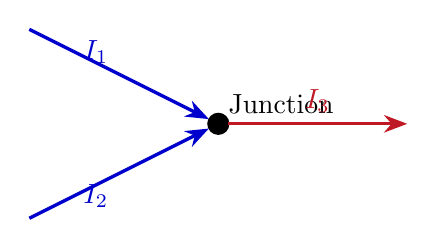
\begin{tikzpicture}[>=Stealth, thick, scale=1.2]
        % Junction point
        \filldraw [black] (0,0) circle (3pt) node[above right] {Junction};
        % Current arrows
        \draw [->, blue!80!black, very thick] (-2, 1) -- (-0.1, 0.05) node[midway, above left] {$I_1$};
        \draw [->, blue!80!black, very thick] (-2, -1) -- (-0.1, -0.05) node[midway, below left] {$I_2$};
        \draw [->, CrimsonRed, very thick] (0.1, 0) -- (2, 0) node[midway, above] {$I_3$};
    \end{tikzpicture}
\end{center}

\begin{formulabox}[Kirchhoff's Current Law]
    \[ \sum I = 0 \quad \implies \quad I_{\text{in}} = I_{\text{out}} \]
    In the diagram above: $I_1 + I_2 = I_3$. \\[0.15cm]
    \textbf{Conservation Law:} Based on the \textbf{Law of Conservation of Charge}.
\end{formulabox}

\subsection{Kirchhoff's Voltage Law (KVL)}
\begin{pyqbox}[PYQ Priority: \textasteriskcentered\textasteriskcentered\textasteriskcentered\textasteriskcentered]
    \textbf{Statement:} The algebraic sum of all branch voltages and emf sources around any closed loop in a circuit is equal to zero.
\end{pyqbox}

\begin{formulabox}[Kirchhoff's Voltage Law]
    \[ \sum V = 0 \]
    \textbf{Conservation Law:} Based on the \textbf{Law of Conservation of Energy}.
\end{formulabox}

\subsection{Thevenin's Theorem}
\begin{pyqbox}[PYQ Priority: \textasteriskcentered\textasteriskcentered\textasteriskcentered\textasteriskcentered\textasteriskcentered\ (Direct PYQ Proof)]
    \textbf{Statement:} Any linear, bilateral two-terminal network consisting of voltage/current sources and resistances can be replaced by an equivalent circuit containing a single voltage source $V_{\text{th}}$ in series with an equivalent resistance $R_{\text{th}}$.
\end{pyqbox}

\begin{center}
    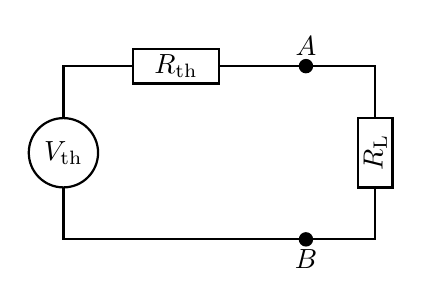
\begin{tikzpicture}[>=Stealth, thick, scale=1.1]
        % Circle for Vth
        \draw (0,0) circle (0.4cm) node {$V_{\text{th}}$};
        \draw (0,0.4) -- (0,1) -- (0.8,1);
        % Resistor Rth
        \draw (0.8,0.8) rectangle (1.8, 1.2) node[midway] {$R_{\text{th}}$};
        \draw (1.8,1) -- (2.8,1);
        % Terminal A
        \filldraw (2.8,1) circle (2pt) node[above] {$A$};
        \draw (2.8,1) -- (3.6,1) -- (3.6,0.4);
        % Resistor RL
        \draw (3.4,-0.4) rectangle (3.8, 0.4) node[midway, rotate=90] {$R_{\text{L}}$};
        \draw (3.6,-0.4) -- (3.6,-1) -- (2.8,-1);
        % Terminal B
        \filldraw (2.8,-1) circle (2pt) node[below] {$B$};
        \draw (2.8,-1) -- (0,-1) -- (0,-0.4);
    \end{tikzpicture}
\end{center}

\begin{formulabox}[Thevenin Values]
    \[ V_{\text{th}} = \text{Open-circuit voltage measured across terminals } AB \]
    \[ R_{\text{th}} = \text{Equivalent resistance looking back into } AB \text{ with active sources deactivated} \]
\end{formulabox}

\subsubsection{Procedure to Find Thevenin Equivalent}
\begin{enumerate}
    \item Remove the load resistance $R_L$ from terminals $A$ and $B$.
    \item Calculate the open-circuit voltage $V_{\text{oc}}$ across terminals $A$ and $B$. This is $V_{\text{th}}$.
    \item Deactivate all independent sources:
    \begin{itemize}
        \item Replace independent voltage sources with a \textbf{short circuit}.
        \item Replace independent current sources with an \textbf{open circuit}.
    \end{itemize}
    \item Calculate the equivalent resistance looking back into terminals $A$ and $B$. This is $R_{\text{th}}$.
    \item Reconnect $R_L$ and compute the load current:
    \begin{formulabox}[Thevenin Load Current]
        \[ I_L = \frac{V_{\text{th}}}{R_{\text{th}} + R_L} \]
    \end{formulabox}
\end{enumerate}

\subsection{Norton's Theorem}
\begin{pyqbox}[PYQ Priority: \textasteriskcentered\textasteriskcentered\textasteriskcentered\textasteriskcentered\ (Direct PYQ Proof)]
    \textbf{Statement:} Any linear, bilateral active two-terminal network can be replaced by an equivalent circuit consisting of a single constant current source $I_N$ in parallel with an equivalent resistance $R_N$.
\end{pyqbox}

\begin{center}
    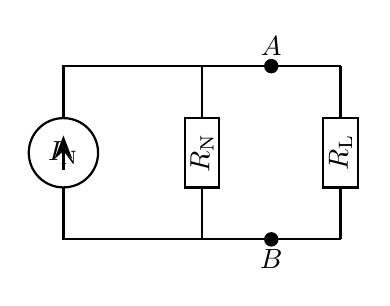
\begin{tikzpicture}[>=Stealth, thick, scale=1.1]
        % Current source IN
        \draw (0,0) circle (0.4cm) node {$I_{\text{N}}$};
        \draw [->, very thick] (0,-0.2) -- (0,0.2);
        \draw (0,0.4) -- (0,1) -- (3.2,1);
        \draw (0,-0.4) -- (0,-1) -- (3.2,-1);
        
        % Resistor RN in parallel
        \draw (1.6,1) -- (1.6,0.4);
        \draw (1.4,-0.4) rectangle (1.8, 0.4) node[midway, rotate=90] {$R_{\text{N}}$};
        \draw (1.6,-0.4) -- (1.6,-1);
        
        % Terminals
        \filldraw (2.4,1) circle (2pt) node[above] {$A$};
        \filldraw (2.4,-1) circle (2pt) node[below] {$B$};
        
        % Load resistor RL
        \draw (3.2,1) -- (3.2,0.4);
        \draw (3.0,-0.4) rectangle (3.4, 0.4) node[midway, rotate=90] {$R_{\text{L}}$};
        \draw (3.2,-0.4) -- (3.2,-1);
    \end{tikzpicture}
\end{center}

\begin{formulabox}[Norton Values]
    \[ I_N = \text{Short-circuit current } I_{sc} \text{ flowing between terminals } AB \]
    \[ R_N = \text{Thevenin resistance } R_{\text{th}} \]
\end{formulabox}

\begin{formulabox}[Norton Load Current]
    \[ I_L = I_N \left( \frac{R_N}{R_N + R_L} \right) \]
\end{formulabox}

\subsection{Thevenin--Norton Conversion}
\begin{formulabox}[Source Transformations]
    \textbf{Thevenin to Norton:}
    \[ I_N = \frac{V_{\text{th}}}{R_{\text{th}}} \]
    \textbf{Norton to Thevenin:}
    \[ V_{\text{th}} = I_N R_N \]
    \textbf{Resistances:}
    \[ R_N = R_{\text{th}} \]
\end{formulabox}

\subsection{Maximum Power Transfer Theorem}
\begin{pyqbox}[PYQ Priority: \textasteriskcentered\textasteriskcentered\textasteriskcentered\textasteriskcentered\textasteriskcentered]
    \textbf{Statement:} Maximum power is transferred from a source network to an adjustable load resistance $R_L$ when the value of the load resistance is equal to the internal resistance $R_s$ (or Thevenin equivalent resistance $R_{\text{th}}$) of the source network.
\end{pyqbox}

\begin{center}
    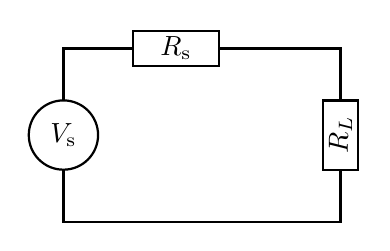
\begin{tikzpicture}[>=Stealth, thick, scale=1.1]
        % Voltage source Vs
        \draw (0,0) circle (0.4cm) node {$V_{\text{s}}$};
        \draw (0,0.4) -- (0,1) -- (0.8,1);
        % Resistor Rs
        \draw (0.8,0.8) rectangle (1.8, 1.2) node[midway] {$R_{\text{s}}$};
        \draw (1.8,1) -- (2.6,1);
        % Load resistor RL
        \draw (2.6,1) -- (3.2,1) -- (3.2,0.4);
        \draw (3.0,-0.4) rectangle (3.4, 0.4) node[midway, rotate=90] {$R_L$};
        \draw (3.2,-0.4) -- (3.2,-1) -- (0,-1) -- (0,-0.4);
    \end{tikzpicture}
\end{center}

\begin{formulabox}[Theorem Condition]
    \[ R_L = R_s \quad \text{or} \quad R_L = R_{\text{th}} \]
\end{formulabox}

\subsubsection{Derivation Framework}
Power delivered to the load $P_L$:
\[ P_L = I^2 R_L = \left( \frac{V_s}{R_s + R_L} \right)^2 R_L \]
To maximize power, set $\frac{dP_L}{dR_L} = 0$:
\[ \frac{d}{dR_L} \left[ \frac{V_s^2 R_L}{(R_s + R_L)^2} \right] = 0 \quad \implies \quad R_L = R_s \]
Substituting $R_L = R_s$ yields the maximum power:
\begin{formulabox}[Maximum Power Formula]
    \[ P_{\text{max}} = \frac{V_s^2}{4R_s} \]
\end{formulabox}

\begin{formulabox}[Efficiency at Max Power]
    \[ \eta = 50\% \]
\end{formulabox}

\subsection{Theorem Comparison Table}
\begin{table}[htbp]
    \centering
    \caption{Key Network Theorem Summaries}
    \vspace{0.2cm}
    \begin{tabular}{lll}
        \toprule
        \textbf{Theorem} & \textbf{Equivalent Form} & \textbf{Key Relation / Output} \\
        \midrule
        \textbf{Thevenin} & Voltage source in series with $R_{\text{th}}$ & $I_L = \frac{V_{\text{th}}}{R_{\text{th}} + R_L}$ \\
        \textbf{Norton} & Current source in parallel with $R_N$ & $I_L = I_N \frac{R_N}{R_N + R_L}$ \\
        \textbf{Max Power} & Load matched to source resistance & $R_L = R_{\text{th}} \implies P_{\text{max}} = \frac{V_{\text{th}}^2}{4R_{\text{th}}}$ \\
        \bottomrule
    \end{tabular}
\end{table}

\newpage
\begin{prioritybox}[Network Theory PYQ Priority]
    Focus first on the following topics:
    \begin{enumerate}[label=\textbf{\arabic*.}]
        \item \textbf{Thevenin's Theorem:} Step-by-step proofs and analytical circuit analysis.
        \item \textbf{Maximum Power Transfer Theorem:} Proof of $R_L = R_{\text{th}}$, calculation of maximum power and $50\%$ efficiency limit.
        \item \textbf{Norton's Theorem:} Parallel equivalence and Norton--Thevenin transformation steps.
        \item \textbf{Kirchhoff's Laws (KCL \& KVL):} Conceptual base and physical conservation principles.
    \end{enumerate}
\end{prioritybox}

\begin{successbox}
    Network Theory Revision Complete! \checkmark
\end{successbox}

\newpage
% =========================================================================
% COMPLETE FORMULA SHEET
% =========================================================================
\section{Entire Electricity \& Magnetism Formula Sheet (Highest Priority)}

This is a comprehensive reference sheet listing all crucial formulas across all four parts. Memorize these!

\subsection{Electrostatics}
\begin{itemize}
    \item \textbf{Electric Field:} $E = \frac{1}{4\pi\epsilon_0}\frac{Q}{r^2}$
    \item \textbf{Electric Potential:} $V = \frac{1}{4\pi\epsilon_0}\frac{Q}{r}$
    \item \textbf{Potential Gradient Relation:} $E = -\frac{dV}{dr} \quad \text{or} \quad \vec{E} = -\nabla V$
    \item \textbf{Dipole Moment:} $p = q(2a)$
    \item \textbf{Potential Due to Dipole:} $V_{\text{dipole}} = \frac{1}{4\pi\epsilon_0}\frac{p\cos\theta}{r^2}$
    \item \textbf{Axial Dipole Electric Field:} $E_{\text{axial}} = \frac{1}{4\pi\epsilon_0}\frac{2p}{r^3}$
    \item \textbf{Equatorial Dipole Electric Field:} $E_{\text{equatorial}} = \frac{1}{4\pi\epsilon_0}\frac{p}{r^3}$
\end{itemize}

\subsection{Magnetostatics}
\begin{itemize}
    \item \textbf{Lorentz Force:} $F = qvB\sin\theta$
    \item \textbf{Force on Wire:} $F = BIL\sin\theta$
    \item \textbf{Biot--Savart Law:} $dB = \frac{\mu_0}{4\pi}\frac{Idl\sin\theta}{r^2}$
    \item \textbf{Infinite Straight Wire Field:} $B = \frac{\mu_0I}{2\pi r}$
    \item \textbf{Circular Coil Axial Field:} $B = \frac{\mu_0NIR^2}{2(R^2+x^2)^{3/2}}$
    \item \textbf{Solenoid Field:} $B = \mu_0 n I$
\end{itemize}

\subsection{Electromagnetic Induction}
\begin{itemize}
    \item \textbf{Induced emf (Faraday's Law):} $e = -N\frac{d\phi_B}{dt}$
    \item \textbf{Self-Induced emf:} $e = -L\frac{dI}{dt}$
    \item \textbf{Self-Inductance of a Solenoid:} $L = \frac{\mu_0N^2A}{l}$
    \item \textbf{Mutual Inductance of Two Solenoids:} $M = \frac{\mu_0N_1N_2A}{l}$
    \item \textbf{Continuity Equation (Charge Conservation):} $\nabla\cdot\vec{J} + \frac{\partial\rho}{\partial t} = 0$
    \item \textbf{Displacement Current:} $I_d = \epsilon_0\frac{d\phi_E}{dt}$
\end{itemize}

\subsection{Network Theory}
\begin{itemize}
    \item \textbf{Ohm's Law:} $V = IR$
    \item \textbf{Thevenin Circuit Load Current:} $I_L = \frac{V_{\text{th}}}{R_{\text{th}}+R_L}$
    \item \textbf{Thevenin--Norton Conversion:} $I_N = \frac{V_{\text{th}}}{R_{\text{th}}} \quad \text{and} \quad R_N = R_{\text{th}}$
    \item \textbf{Maximum Power Transfer Condition:} $R_L = R_{\text{th}}$
    \item \textbf{Maximum Power Output:} $P_{\text{max}} = \frac{V_s^2}{4R_s}$
\end{itemize}

\begin{successbox}
    All E\&M One-Shot Revision Content Successfully Transformed into LaTeX! \checkmark
\end{successbox}

\end{document}
